\documentclass[a4paper, 11pt]{article}
\usepackage[top=2cm, bottom=3cm, left = 2cm, right = 2cm]{geometry} 
\geometry{a4paper} 
\usepackage{textcomp}
\usepackage{graphicx} 
\usepackage{amsmath,amssymb}  
\usepackage{bm}  
\usepackage{memhfixc} 
\usepackage{fancyhdr}
\usepackage{enumerate}
\usepackage{tikz}
\usepackage{float}
\usepackage{booktabs}
\usepackage{listings}
\usepackage[framed]{ntheorem}
\pagestyle{fancy}
\setlength{\headheight}{14pt}
\addtolength{\topmargin}{-2pt}
\theoremstyle{nonumberplain}
\newtheorem{definition}{Definition}

\lstset{basicstyle=\ttfamily,
  showstringspaces=false,
  commentstyle=\color{red},
  keywordstyle=\color{blue}
}

\title{Virtual Machine Environment}
\author{Hossein Afkar}
%\date{}

\begin{document}
\maketitle
% \tableofcontents

\section{Environment}
In this computer assignment, we will demonstrate the container communication
notions. The container runtime of choice for this assignment is docker and the
communication is done using the gRPC protocol. For this assignment,
we used the go programming language. Our goal was to create a client and server
for transferring messages with their respected timestamps in a gRPC call.
To achieve this first, we must write a proto file that describes the functions
that can be called between clients and servers.

\begin{lstlisting}[language=go]
syntax = "proto3";
import "google/protobuf/timestamp.proto";

option go_package = "github.com/alphamaster32/lightship/proto";

package MessageService;

service MessagePasser {
    rpc SendMessage(Hello) returns (Hello) {}
}

message Hello {
    string msg = 1;
    google.protobuf.Timestamp ts = 2;
}

\end{lstlisting}
The \textit{SendMessage} function passes a struct to the callee with a string
and a timestamp. To compile this protobuf file and make the templates we must
first generate the code templates using \textit{make proto} which in turn uses
the written GNU Make to make these templates. After that, we must implement
these functions defined in the interfaces for the server as described in the
\textit{server.go} source files.

\begin{lstlisting}[language=go]
type grpcServer struct {
	pb.UnimplementedMessagePasserServer
}

func (s *grpcServer) SendMessage(ctx context.Context,
	in *pb.Hello) (*pb.Hello, error) {
	fmt.Print(in.Msg, "\t")
	fmt.Println(in.Ts.AsTime())
	return &pb.Hello{
		Msg: "Hello World! From Server",
		Ts:  timestamppb.Now(),
	}, nil
}
\end{lstlisting}
This code sends the string message with the time stamp to the client.
After this we must make a request in the server in the client
\begin{lstlisting}[language=go]
for {
    conn, err := grpc.Dial(port_str,
    grpc.WithTransportCredentials(insecure.NewCredentials()))
    if err != nil {
        return err
    }
    defer conn.Close()
    c := pb.NewMessagePasserClient(conn)

    ctx, cancel := context.WithTimeout(context.Background(), time.Second)
    defer cancel()

    r, err := c.SendMessage(ctx, &pb.Hello{
        Msg: "Hello World! From Client",
        Ts:  timestamppb.Now(),
    })
    if err != nil {
        return err
    }

    fmt.Print(r.Msg, "\t")
    fmt.Println(r.Ts.AsTime())
    time.Sleep(10 * time.Second)
}
\end{lstlisting}
The client loops forever and calls the SendMessage gRPC function and sends in
the Hello struct defined in the proto file. The server then receives this
information prints it out and sends another Hello struct to the caller.
After this, the clients receive the Hello structs and print their contents.
Here is a figure representing a sample output of the client-server output:
\begin{figure}[H]
    \centering
    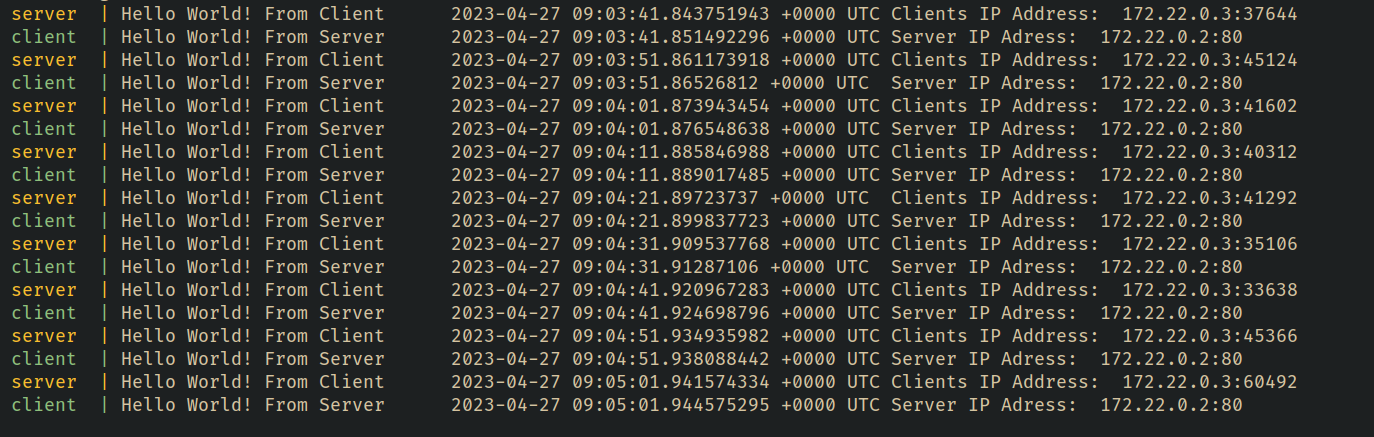
\includegraphics[width=1.0\textwidth]{output.png}
    \caption{Sample output of the lightship client and server using
    docker-compose}
    \label{fig:output}
\end{figure}
This output is provided by the docker-compose. The command used for the
invocation of the docker-composes is stated as follows:
\begin{lstlisting}[language=bash]
docker-compose up --no-deps --build
\end{lstlisting}
The \textit{Dockerfile}s and the \textit{docker-compose.yml} file is included
in the project directory. The overall description of docker environment is
two client and server containers. The client will loop forever and requests
a gRPC call every 10 seconds. IP is assigned statically to the both server and
client containers. The server ip is passed as an environment variable to 
the client. \\
The source code is included in the project files.
Tools that are used in this project report are listed below:
\begin{itemize}
    \item golang
    \item protoc with golang plugin
    \item docker
    \item docker-compose
\end{itemize}

\section{Conculsion}
In this project we made a gRPC connection between two containers over a
network bridge. In order to do this we made use of the golang and the proto
compiler to define a gRPC procedure call. In the last assignment we made a
connection between two virtual machines. Connection between virtual machines
was done using a simple tcp socket and \textit{lxc} virtual machines using
\textit{--vm} command. The main difference between the aforementioned methods
was the data encoding in the socket calls. gRPC data is sent over a tcp socket
with extra data encodings (HTTP/2). gRPC handles connection closure gracefully
but the tcp method used in the last assignment will fail on the closed socket
and will not retry. Also the network bridge between the virtual machines is
passed on a fully virtualized network adapter but in the container world this
is handled using \textit{namespaces}. Overall the gRPC is battle tested
protocol for the communication on the network channels between various hosts
on different network and with different network capabilities.




% \bibliographystyle{abbrv}
% \bibliography{references}  % need to put bibtex references in references.bib 
\end{document}
